\section{Overbelægning}\label{sec:overbelaegning}
Overbelægning opstår, når en afdeling har en belægningsprocent på over 85. I perioden fra år 1996 til 2011 er sengepladserne på de danske hospitalsafdelinger reduceret med 30 \%, for således at tilnærme sig en fuld udnyttelse af ressoucerne. Herunder udnyttelse af de tilgængelige sengepladser på hospitalsafdelingerne samt optimering af sundhedspersonalets arbejdstid \cite{Madsen2014}. 

Antallet af indlagte patienter varierer hver måned, hvorfor tilgængeligheden af sengepladser ligeledes varierer. På \autoref{fig:overbelaegning_ran} er det illustreret, hvordan de forskellige afdelinger  på tværs af Danmark oplever overbelægning i januar måned år 2015.

\begin{figure}[H]
\centering
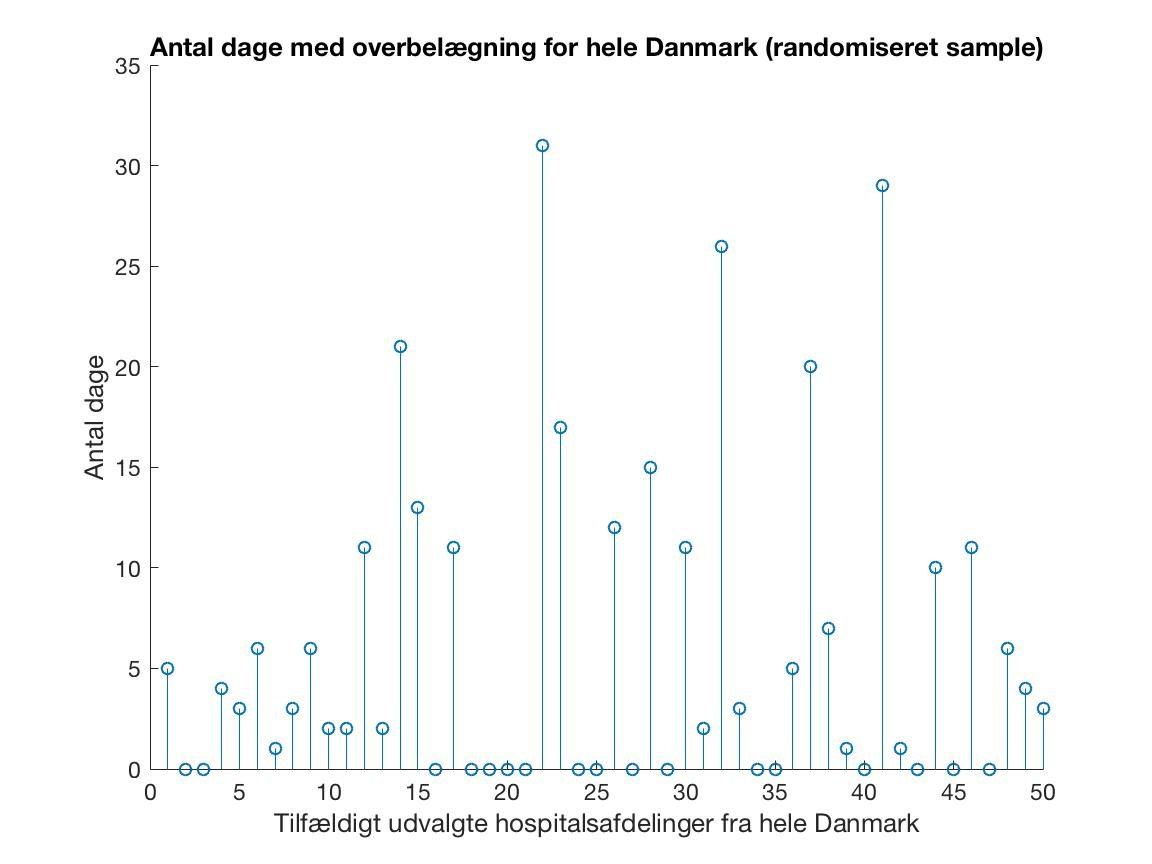
\includegraphics[width=1\textwidth]{figures/overbelaegning_ran}
\caption{Illustrerer antal dage med overbelægning på 50 tilfældige hospitalsafdelinger fra hele Danmark. De tilfældige data er taget fra januar måned år 2015. \cite{SDS2015}} 
\label{fig:overbelaegning_ran}
\end{figure}

\noindent
Det ses af \autoref{fig:overbelaegning_ran}, at der er en tendens til overbelægning på flere hospitalsafdelinger i Danmark. Ud af de 50 tilfældige hospitalsafdelinger har 35 af afdelingerne oplevet overbelægning i januar måned. Herudover ses det af figuren, at nogle afdelinger har haft overbelægning op til 31 dage, hvilket svarer til, at afdelingen har haft overbelægning alle dage i januar måned.

\begin{figure}[H]
\centering
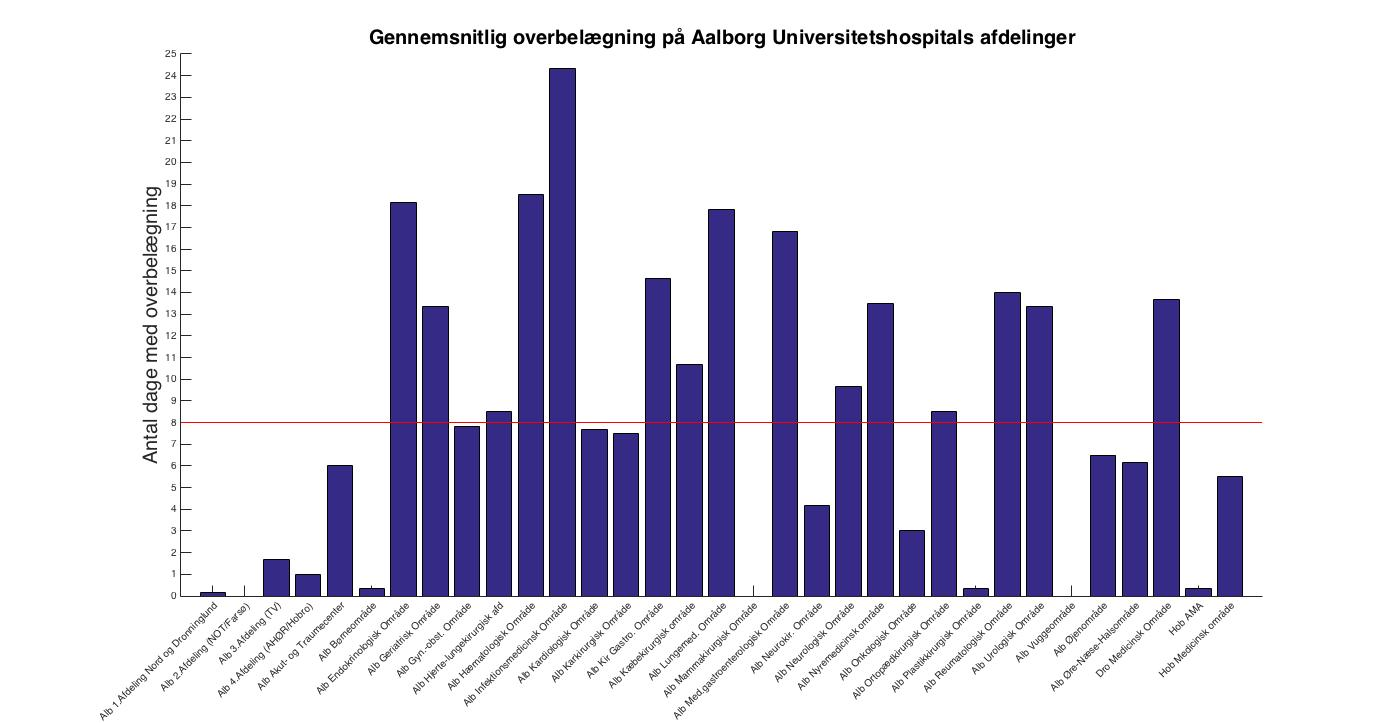
\includegraphics[width=1\textwidth]{figures/overbelaegning_AUH}
\caption{Søjlerne illustrerer gennemsnittet af antal dage med overbelægning på Aalborg universitetshospitalsafdelinger fra januar til juni år 2015. \cite{SDS2015} Den røde linje viser gennemsnittet af søjlerne. Denne er beregnet til en gennemsnitlig overbelægning på 8,29 dage.}
\label{fig:overbelaegning_AUH}
\end{figure}

\noindent
Det fremgår af \autoref{fig:overbelaegning_AUH}, at der ligeledes er en tendens til overbelægning på Aalborg universitetshospital. Der ses variation i antal dage med overbelægning på afdelingerne, dog ses overbelægning på 30 ud af 33 afdelinger i perioden fra januar til juni år 2015. På ambulatorisk infektionsmedicinsk område opleves en gennemsnitlig overbelægning på 24 dage, hvorimod eksempelvis ambulatorisk 2. afdeling ikke berøres af overbelægning. Gennemsnitlig er der en overbelægning på 8 dage for afdelingerne i perioden januar til juni år 2015.

